%!TEX root = ../thesis.tex
% ******************************* Thesis Appendix A ****************************
\cleardoublepage
\chapter{Univariate distribution fitting}
\label{apx:A}
%*******************************************************************************

This appendix recalls the main methods to infer a univariate distribution considering a $n$-sized i.i.d sample $X_n = \left\{x^{(1)}, \dots, x^{(n)}\right\} \in \R^{n}$. 
The goal is to use this finite set of observations of the random variable $X$ to approach its underlying distribution by an estimated distribution.
The inference techniques are split into two main groups, the methods assuming that the underlying distribution belongs to a family of parametric distributions are called parametric. 
Otherwise, the fitting method falls into the nonparametric group. 
Nonparametric methods often require a larger amount of data but allow more flexibility. 
In fact, nontrivial distributions (e.g., multimodal) might be easier to model using nonparametric approaches.
To assess the quality of this estimation regarding the sample, a panel of goodness-of-fit methods are proposed \elias{add ref}, this appendix recalls a few of them. 
Note that the following tools can be used to estimate the marginals of a multivariate distribution.

%============================================================%
%============================================================%
\section*{Main parametric methods}
%============================================================%
%============================================================%

%============================================================%
\subsection*{Moments method}
%============================================================%
The moment's method aims at looking for a parametric distribution with density $f_X(\btheta)$, whose first moments (e.g., $m(\btheta)$ and $\sigma^2(\btheta)$) match 
the empirical moments of the sample $X_n$ (e.g., $\what{m}_{X_n}$ and $\what{\sigma}^2$). After computing the empirical moments: 
\begin{equation}
    \what{m}_{n} = \frac1n \sum_{i=1}^{n} x^{(i)}, \qquad \what{\sigma}^2_n = \frac{1}{n-1} \sum_{i=1}^{n} \left(x^{(i)} - \what{m}_{X_n}\right)^2,
\end{equation} 
one can solve the system of equations $\left(m(\btheta) = \what{m}_{n}; \ \sigma^2(\btheta) = \what{\sigma}_n^2\right)$ to determine the optimal set of parameters $\btheta$ in this situation. 
Some families of distributions are more suited to this method (i.e., ) because of the analytical expression of their moments. 
Moreover, this technique is sensitive to the possible biases in the estimation of the sample moments.

%============================================================%
\subsection*{Maximum likelihood estimation}
%============================================================%
Maximum likelihood estimation (MLE) is a popular alternative to the moments method. 
Similarly, it aims at maximizing a given correspondence metric between the dataset $X_n$ and a parametric distribution with density $f_X(\btheta)$.
This metric is the \textit{likelihood} function, defined as:
\begin{equation}
    \mathcal{L}(\btheta|X_n) = \prod_{i=1}^{n} f_X(x^{(i)}; \btheta), 
\end{equation}
with the PDF taking the set of parameters $\btheta$ written: $f_X(x^{(i)}; \btheta)$. For numerical reasons, the optimization is often performed on the natural logarithm of the likelihood function, called \textit{log-likelihood}. 
The goal is then finding the optimal vector $\what{\btheta}^*$ of parameters minimizing the following expression: 
\begin{equation}
    \what{\btheta}^* = \argmin_{\btheta \in \iD_{\btheta}} \left(-\sum_{i=1}^{n} \ln(f_X(x^{(i)}; \btheta)) \right).
\end{equation}

Remark that the quick analytical results from the moment method can be used as a starting point of the MLE optimization. 
\elias{Asymptotic behaviors of this method are described in: add ref}
\elias{This method can be applied to censored data in the field of survival analysis. Add ref}

\begin{example}
    \label{ex:mle}
    Considering a small set of observations $X_n = \{1, 2, 3, 4, 6\}$, the following figure xx represents 
    \begin{figure}[H]
        \centering
        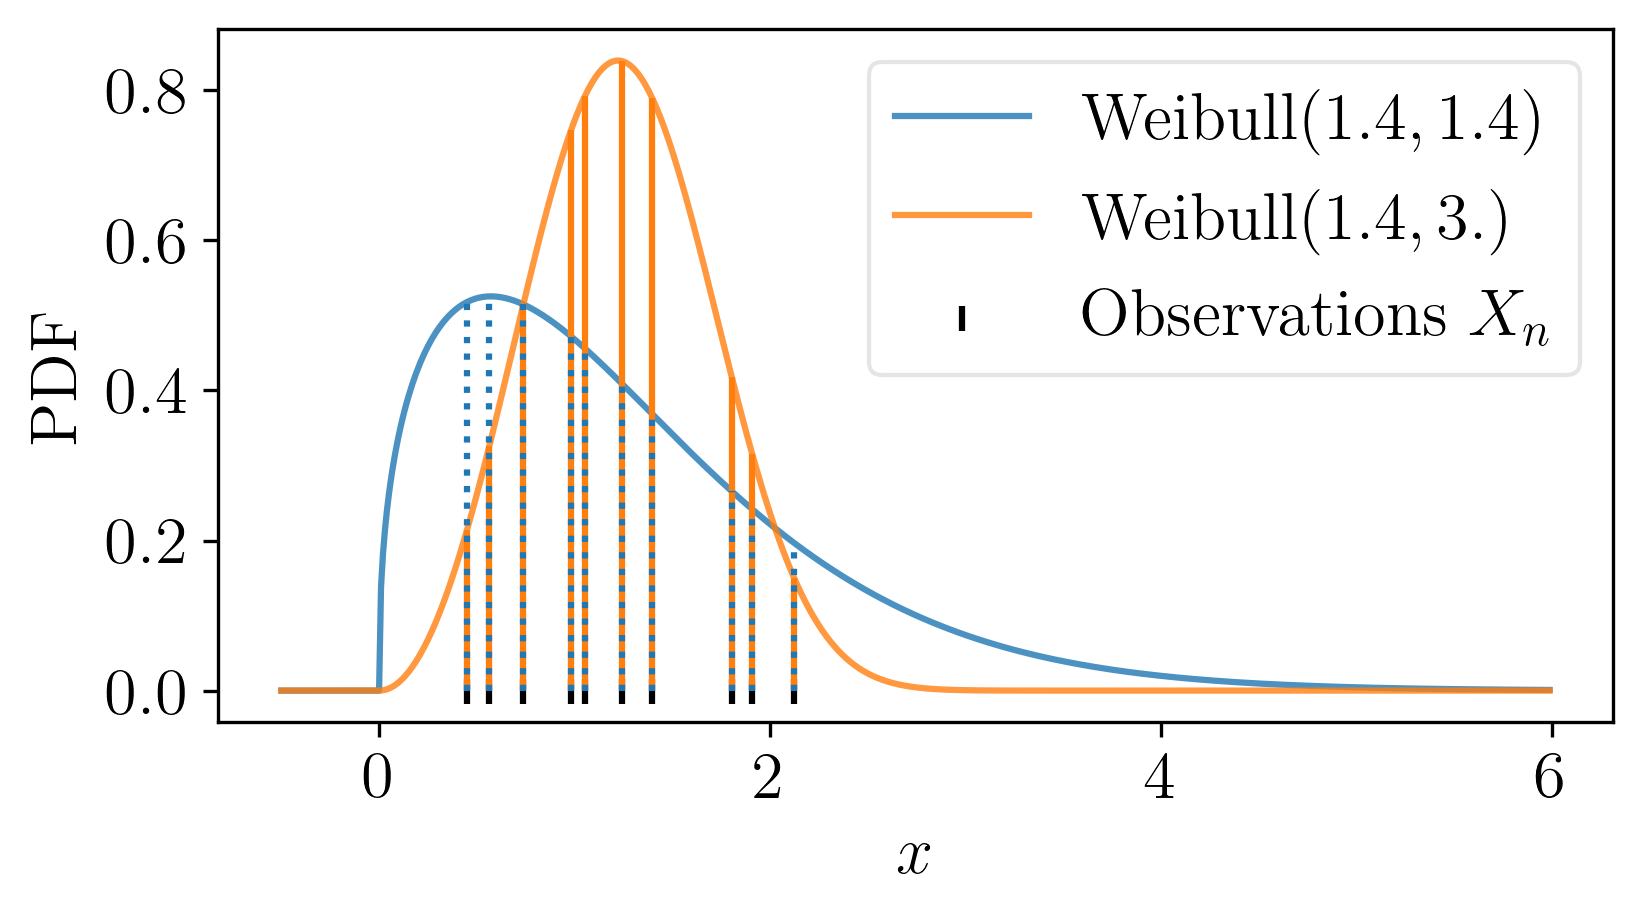
\includegraphics[width=0.5\textwidth]{../numerical_experiments/chapter1/figures/MLE.png}
        \caption{Adequation of two different Weibull models using their likelihood with a sample of observations (black crosses). }
        \label{fig:MLE}
    \end{figure}
\end{example}


%============================================================%
%============================================================%
\section*{Main nonparametric methods}
%============================================================%
%============================================================%


%============================================================%
\subsection*{Empirical CDF and histogram}
%============================================================%
The empirical CDF is a cumulative stair-shaped representation of the sorted sample $X_n$:
\begin{equation}
    \what{F}_X(x) = \frac1n \sum_{i=1}^{n} \1_{\left\{x^{(i)} \leq x\right\}}.
\end{equation}

A histogram consists of sorting and gathering the observations in a sample $X_n$ into a finite number of categories. 
These categories are called bins and each regroups the same number of observations (identical binwidth). 
The number of bins is the only tunning parameter of this method. 
Its definition has a great impact on the visual consistency of the plot, therefore, many rules exist to define it.
Note that the empirical CDF can be seen as a cumulative histogram with the number of bins equal to the number of observations.


%============================================================%
\subsection*{Kernel density estimation}
%============================================================%
Kernel density estimation (KDE) is a nonparametric method, it estimates a PDF by weighing a sample of observations $X_n$ with kernels.  
After setting a kernel $k: \R \rightarrow \R_+$ and a scaling parameter $h>0$, also called bandwidth, the kernel density estimator is defined as:
\begin{equation}
    \what{f}_X(x) = \frac{1}{n h}\sum_{i=1}^{n} k\left(\frac{x - x^{(i)}}{h}\right)
\end{equation}

Different types of kernels are used for KDE, such as the uniform, triangular, squared exponential or Epachnikov. 
The choice of bandwidth results in a bias-variance trade-off, that has been extensively discussed in the literature \citep{wand_jones_1994_kde}.

\begin{example}
    \label{ex:kde}
    Considering a small set of observations $X_n = \{1, 2, 3, 4, 6\}$, the following figure xx represents three fits obtained by. 
    \begin{figure}[H]
        \centering
        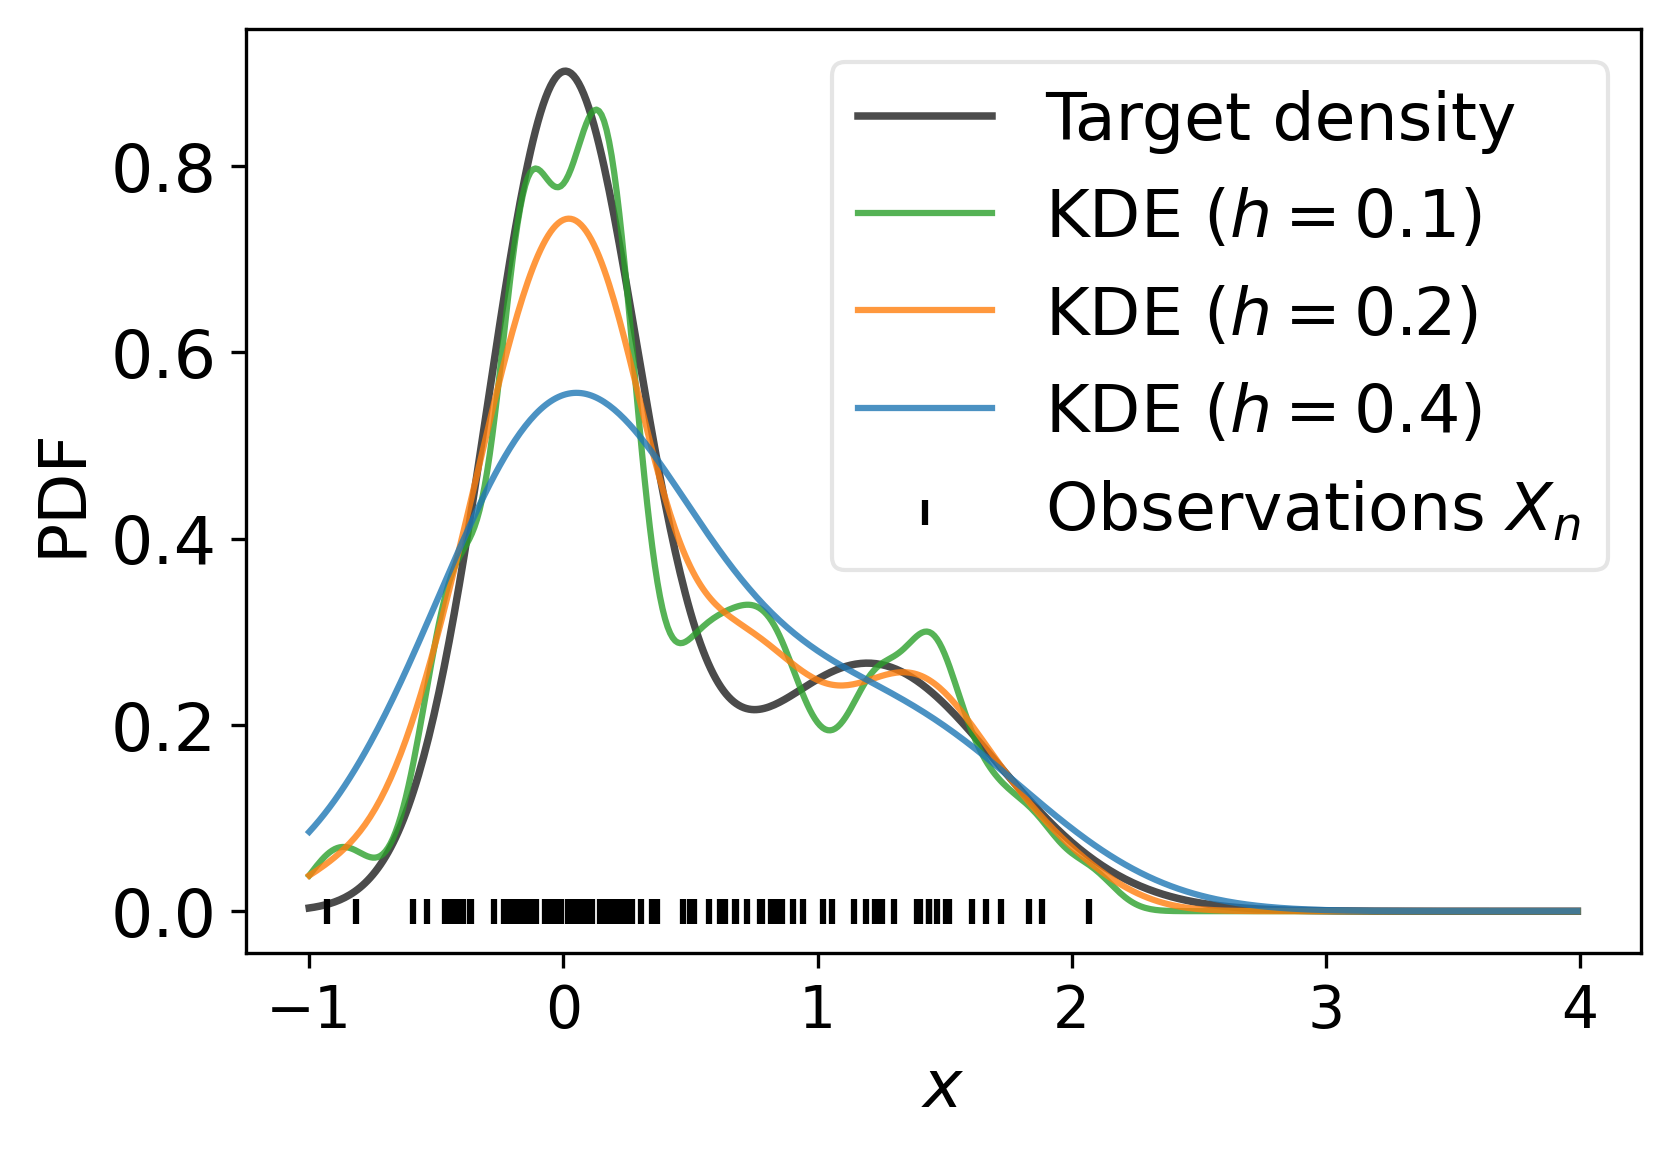
\includegraphics[width=0.5\textwidth]{../numerical_experiments/chapter1/figures/KDE.png}
        \caption{Fit of a bimodal density by KDE using different tuning parameters.}
        \label{fig:KDE}
    \end{figure}
\end{example}

%============================================================%
%============================================================%
\section*{Main goodness-of-fit methods}
%============================================================%
%============================================================%

%============================================================%
\subsection*{Penalized likelihood criteria}
%============================================================%
Two quantitative goodness-of-fit criteria are commonly used to assess parametric inference: the \textit{Akaike information criterion} (AIC) and the \textit{Bayesian information criterion} (BIC). 
The likelihood as a goodness-of-fit criterion should only be applied to the same family of distributions. 
Otherwise, the comparison would unfairly advantage distributions with a large number of degrees of freedom.
The two following criteria are metrics based on the likelihood with a correction related to the number of degrees of freedom of the distribution. 
Moreover, let us remember that more flexible models will require more data to provide a robust estimation. 

The AIC and BIC are expressed as follows:
\begin{equation}
    \textrm{AIC} = \frac{-2 \ln\left(\mathcal{L}(\btheta|X_n)\right)}{n} + \frac{2 q}{n},\qquad
    \textrm{BIC} = \frac{-2 \ln\left(\mathcal{L}(\btheta|X_n)\right)}{n} + \frac{q \ln(n)}{n},
\end{equation}
with the likelihood $\mathcal{L}(\btheta|X_n)$ and the number of distribution's number degrees of freedom denoted $q$.
The second term adds a penalty depending on the number of parameters. 
The best inference will be given by the model with the smallest AIC or BIC. 
Note that an additional correction can be applied in a small data context.

%============================================================%
\subsection*{Kolmogorov-Smirnov adequacy test}
%============================================================%



%============================================================%
\subsection*{Quantile-quantile plot}
%============================================================%

The quantile-quantile plot (also called QQ-plot) is a graphical tool providing a qualitative check of the goodness of fit.
It compares the CDF of the fitted model with the empirical CDF of the sample $X_n$.
To do so, it represents a scatterplot of the empirical quantiles (i.e., the ranked observations), against the quantiles of the fitted model at the levels 
$\left\{\alpha^{(i)}\right\}_{i=1}^n = \left\{\what{F}_X(x^{(i)})\right\}_{i=1}^n$.
The following \fig{fig:qqplot_kde} is a QQ-plot of the model fitted in \elias{Example xx}. The closer the scatter plot gets to the first bisector line the better the fit is.

\begin{figure}[ht]
    \centering
    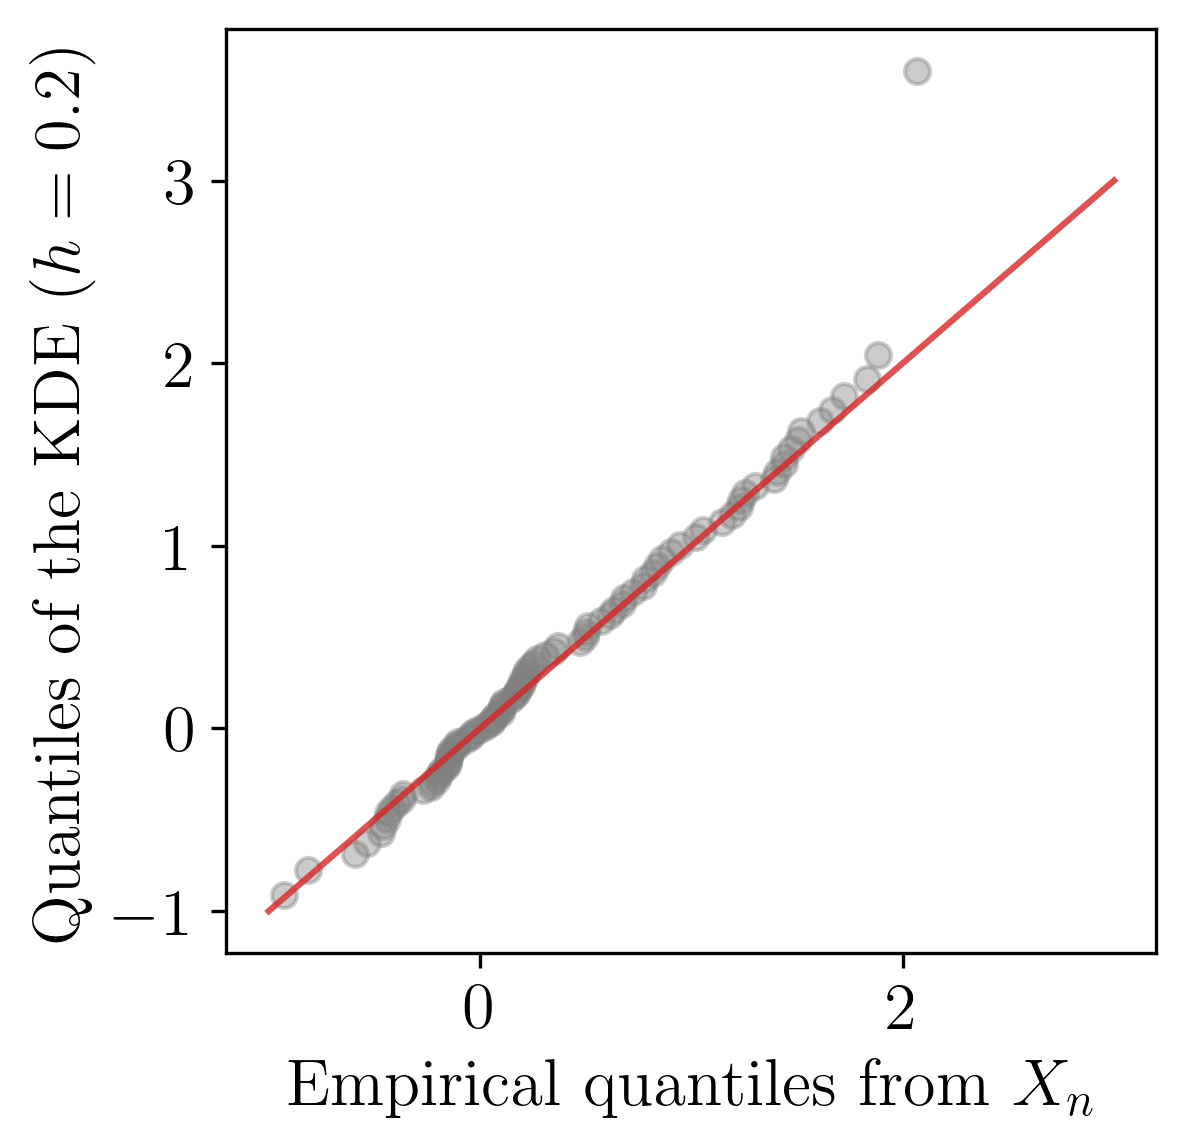
\includegraphics[width=0.5\textwidth]{../numerical_experiments/chapter1/figures/qqplot.png}
    \caption{QQ-plot between the data from Example \ref{ex:kde} and a KDE model.}
    \label{fig:qqplot_kde}
\end{figure}



